\section{Reagent}\label{sec:reagent}

The \textit{Reagent} system allows us a way to hook into the content that is
shown within the Electron framework discussed in Section~\ref{sec:cais}. The
system is broken up into two components, a central server and then the clients.
The central server is used to handle communication from the clients and the
larger CAIS architecture, as well as store information coming from the clients
for reference. This information includes the type of semantic elements exist on
the page, as well as an event stack for recorded user interactions within any
webview. Communication between the server and the clients is handled by using
websockets which facilitates real-time communication of data. To handle requests
from the CAIS, the server implements a RESTful API. The client are inserted as a
transparent layer on top of any opened webview within the system.  This
transparent layer then sets up a connection back to the central server, and then
semantically parses the page using standard DOM traversal via JavaScript
to identify key HTML structures with which a user
might interact with (e.g. a table or a plot), and uses this information to bind
appropriate event handlers to listen for user interactions, as well as for any
changes to the page's content. More specifically,

\begin{enumerate}
    \item Electron pre-loads the \textit{Reagent} system on top of the webview, and injects a websocket connection allowing it to communicate with the open webview and receive JSON-formatted events into an event buffer.
    \item Electron emits a ``DOM Ready" event to signal that the page has finished loading, whereupon \textit{Reagent} scans the page to see if it can detect any major HTML elements it should parse and bind to (e.g. a table).
    \item \textit{Reagent} injects additional code specific to the detected HTML elements that binds event listeners to these elements as well as assigning each a UUID --- an approach that makes \textit{Reagent} readily extensible to new types of elements. (We have implemented domain-independent layers designed for general tables and for plot.ly plots, and allow for domain specific layers as well.)
    \item Next, \textit{Reagent} creates a MutationObserver\footnote{https://mzl.la/1exU78d} to watch for any changes to the page. If changes are detected, it performs any necessary re-injections and re-bindings to ensure that all relevant elements remain instrumented.
    \item Finally, \textit{Reagent} sets up a listener such that if the webview
    is closed, the client disconnects and the server is alerted.
\end{enumerate}

This sequence of events is illustrated within Figure~\ref{fig:reagent}. As an example, we discuss how the
Reagent system would bind to a HTML table and the sorts of queries it would allow for from the user. A perfect data table
is made up of some number of columns and rows where the first row, if marked with the ``th'' tag, should be viewed
as a header row with labels for the columns, and then all subsequent rows marked with the ``td``` tag as data. Reagent
scans the table, generating a list of the column names and some simple heuristics about the structure of the table. Next,
assuming that Reagent has never seen a table on this site before, it first takes all of the headers and attempts to
normalize them as appropriate for its datatype using NLTK and WordNet. Take for example, a column labelled ``won''
for a column with numeric information. Here, the system first casts the word to the present tense of the verb (``win''),
and then pluralizes on its noun form (``wins''), giving us a title more likely to be said by humans. From here, we then
use WordNet to find the variations of the word (on both its noun and verb forms) and add them as entities, if missing,
to Watson Assistant to be used for intent classification on future queries.
Finally, the system binds listeners for user interaction, which in the case of a simple table would be if a user clicks on
a cell in a table or leaves their mouse hovering over it for greater than a second. For any interaction, the client
communicates with the server, which saves a JSON object of the interaction which contains what webview it occurred in,
generated reagent UUID of the element, what row/column the cell was in, contents of the cell, and the type of interaction
it was (e.g. mouseover or click).

During the scan of HTML elements, the system is capable of taking advantage of
content added for accessibility reasons. For example, in
Fig.~\ref{fig:screenshot}, the column for ``appearances'' was labelled ``APP''.
\textit{Reagent} identifies tags that may indicate more human-friendly terms,
such as tooltips that reveal explanatory text when a user hovers over an
element, and uses approximate text matching to infer likely associations where
possible.
In cases where the system is unable to disambiguate the semantic information, it
solicits a definition from the user. For example, with the ESPN table, the
system would ask the user (via synthesized voice) to mouse over ``the column
labeled  \textit{A}'' and state what is the attribute. Upon hearing ``Assign
attribute \textit{assists} to this column", \textit{Reagent} stores the
mapping in a dictionary, whereupon it becomes available to any subsequently
accessed bound elements on the same webpage or host site.

\begin{figure}
\centering
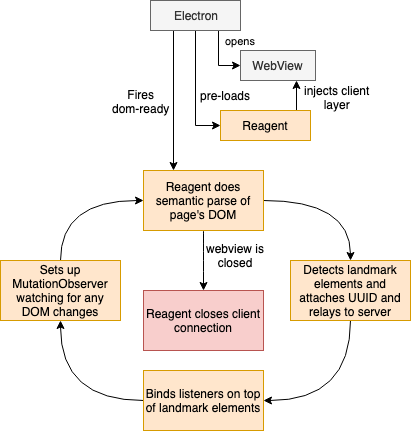
\includegraphics[width=0.45\textwidth]{chapters/03_reagent/figures/reagent.png}
\caption{Flowchart of the Reagent System.}
\label{fig:reagent}
\end{figure}

Through the transparent layer and central server described above, \textit{Reagent} enables
the executor to handle a wider range of queries that pertain to references
to the content within open webviews. At its most basic layer, the user can
query the system for the contents of the full table, what are the columns in a
table, as well as asking queries about statistics (e.g. max, min, or average)
of any given column. By capturing the interactions, it then allows the system
to handle queries that are for relative locations within the interacted with
element. For example, Figure~\ref{fig:screenshot} illustrates the state of the
display after the user has opened an ESPN football team roster webpage and
asked the system ``Show in a new table rows where \textit{appearances} are
greater than 35.''. Equivalently, the user might have asked ``Show in a new
table rows with this column greater than this.'' while pointing to a cell
under the column `APP' with the value of 35.\footnote{For a fuller set of
capabilities that includes query, sorting, and simple analytics like averaging,
a link to a demo video is available at \url{https://bit.ly/20GKvez}}.
